\documentclass[a4paper,11pt]{article}
\usepackage[ngerman]{babel}
\usepackage[ansinew]{inputenc}
\usepackage{geometry}
\usepackage{graphicx}
\usepackage{ulem}
\usepackage{listings}
\usepackage{color}

\geometry{top=20mm, left=30mm, right=30mm, bottom=20mm}
\parindent 0pt
\lstset{language=SQL} 
\lstset{tabsize=4}
\lstset{showstringspaces=false}


\title{Dokumentation zum Datenbankprojekt}
\author{Katharina Chowanski / Marvin Kleinert / Marius Schidlack}  
\date{\today}

\begin{document}
\maketitle 

\section*{Iteration 1: Modellierung}
\subsection*{1. Entity-Relationship-Modell}
\begin{figure}[htbp]
	\centering
		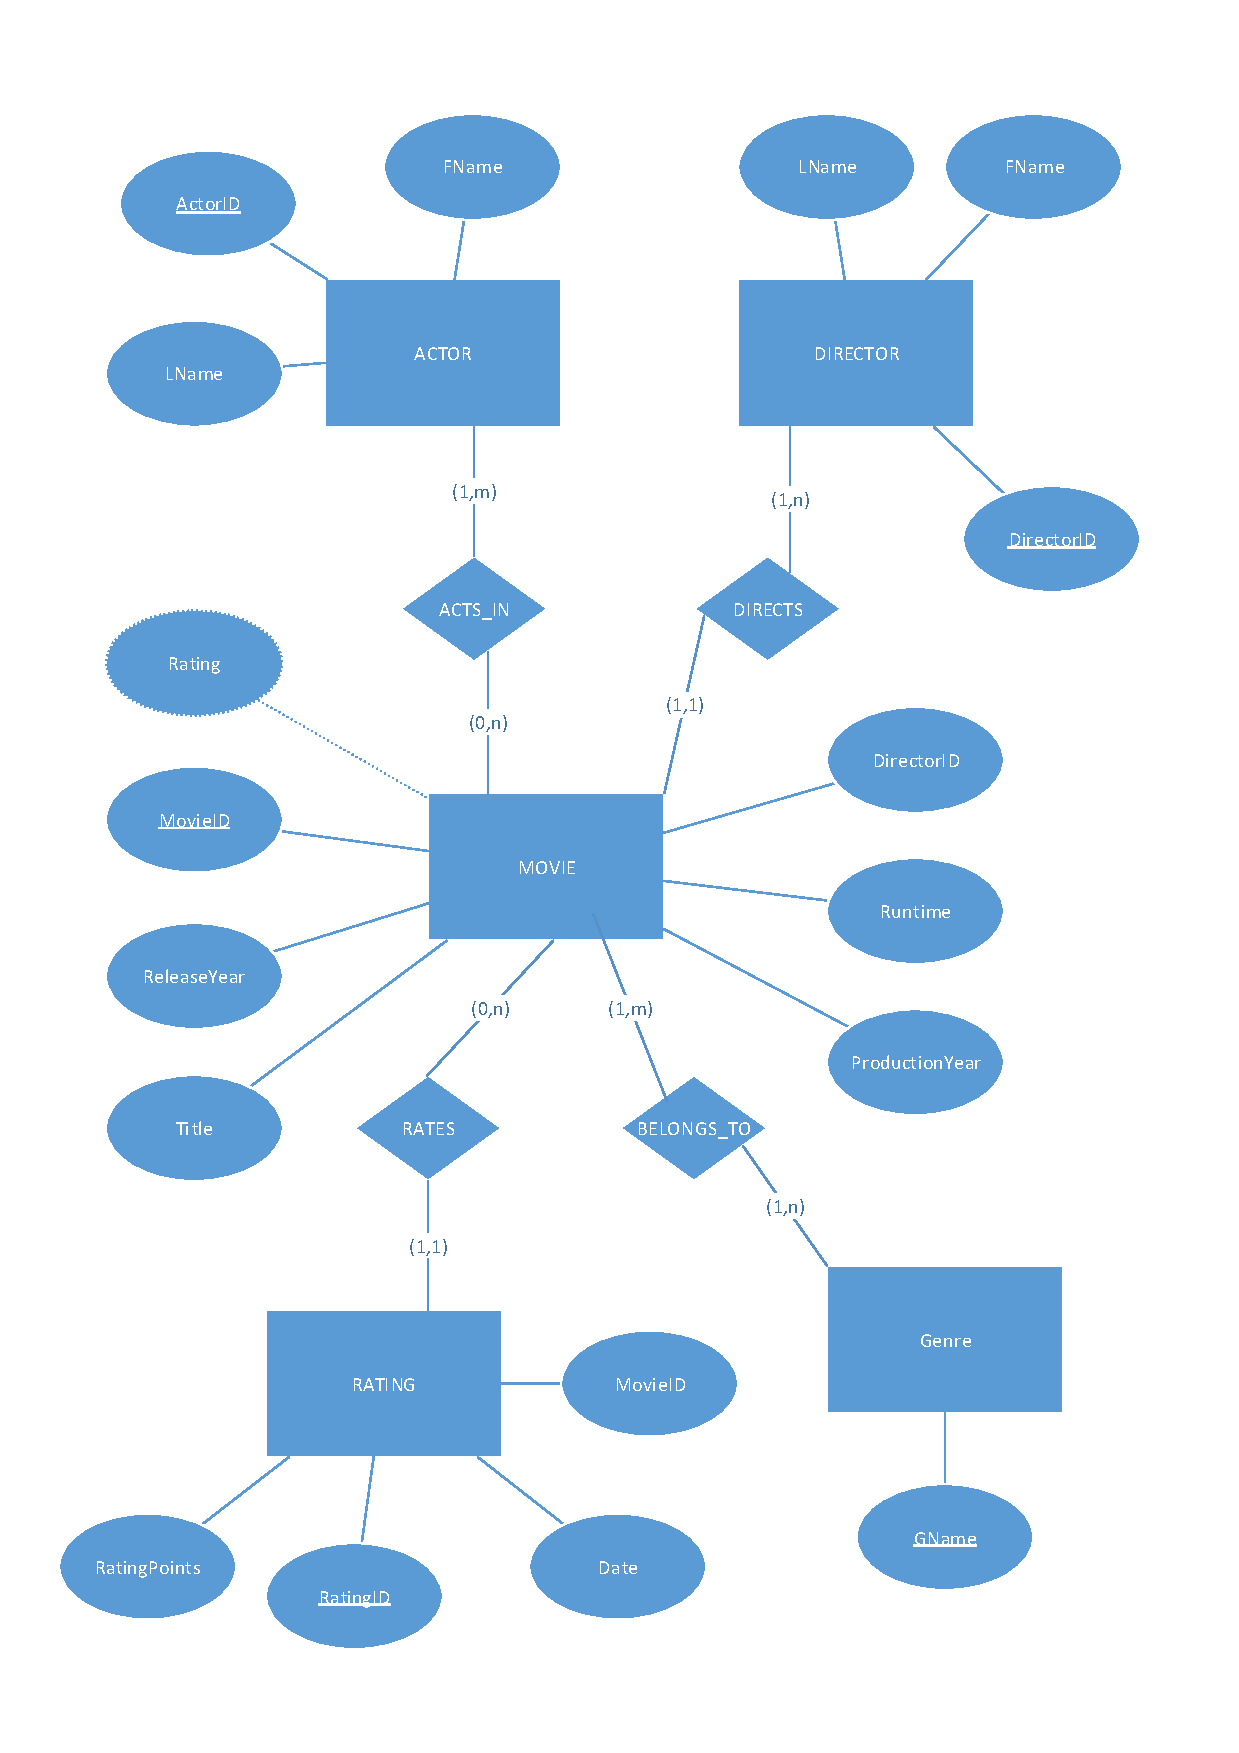
\includegraphics[width=0.85\textwidth]{MoviesER_Portrait.pdf}
	\label{fig:MoviesER}
\end{figure}

<<<<<<< HEAD
\item Relationales Modell \\[0.5cm]
MOVIE (Title: varchar(255); \uline{MovieID}: int8; ReleaseYear: interval YEAR; ProductionYear: interval YEAR; Runtime: int4; DirectorID: int8; Rating: float4)\\[0.5cm]
ACTOR (\uline{ActorID}: int8; FName: varchar(255); Lname: varchar(255))\\[0.5cm]
DIRECTOR (\uline{DirectorID}: int8; FName: varchar(255); LName: varchar(255))\\[0.5cm]
RATING (\uline{RatingID}: int8; Date: date; RatingPoints: int4; MovieID: int8)\\[0.5cm]
GENRE (\uline{GName}: varchar(255))\\[0.5cm]
ACTS\_IN (\underline{\dashuline{MovieID}}: int8; \underline{\dashuline{ActorID}}: int8)\\[0.5cm]
BELONGS\_TO (\underline{\dashuline{GName}}: varchar(255); \underline{\dashuline{MovieID}}: int8)\\[0.5cm]
=======
\subsection*{2. Relationales Modell}
MOVIE (Title: string; \uline{MovieID}: int; ReleaseYear: int; ProductionYear: int; \\Runtime: int; DirectorID: int; Rating: float)\\[0.5cm]
ACTOR (\uline{ActorID}: int; FName: string; Lname: string)\\[0.5cm]
DIRECTOR (\uline{DirectorID}: int; FName: string; LName: string)\\[0.5cm]
RATING (\uline{RatingID}: int; Date: date; RatingPoints: int; MovieID: int)\\[0.5cm]
GENRE (\uline{GName}: string)\\[0.5cm]
ACTS\_IN (\underline{\dashuline{MovieID}}: int; \underline{\dashuline{ActorID}}: int)\\[0.5cm]
BELONGS\_TO (\underline{\dashuline{GName}}: string; \underline{\dashuline{MovieID}}: int)
>>>>>>> f38e48f7e0f459601f6e746e08ba378863513dba

\subsection*{3. CREATE-Statements}
\begin{lstlisting}
CREATE TABLE MOVIE 
(Title				varchar(255) NOT NULL,
MovieID				int8 NOT NULL,
ReleaseYear			interval YEAR,
ProductionYear			interval YEAR,
Runtime				int4,
DirectorID			int8 NOT NULL,
Rating				float4,
PRIMARY KEY (MovieID),
FOREIGN KEY (DirectorID) REFERENCES DIRECTOR (DirectorID)
);

CREATE TABLE ACTOR
(ActorID			int8 NOT NULL,
FName				varchar(255),
LName				varchar(255),
PRIMARY KEY (ActorID)
);

CREATE TABLE DIRECTOR
(DirectorID			int8 NOT NULL,
FName				varchar(255),
LName 				varchar(255),
PRIMARY KEY (DirectorID)
);

CREATE TABLE RATING
(RatingID			int8 NOT NULL,
Date				date,
RatingPoints			int4,
MovieID				int8 NOT NULL,
PRIMARY KEY (RatingID),
FOREIGN KEY (MovieID) REFERENCES MOVIE (MovieID)
);

CREATE TABLE GENRE
(GName				varchar(255) NOT NULL,
PRIMARY KEY (GName)
);

CREATE TABLE ACTS_IN
(MovieID			int8 NOT NULL,
ActorID				int8 NOT NULL,
PRIMARY KEY (MovieID, ActorID),
FOREIGN KEY (MovieID) REFERENCES MOVIE(MovieID),
FOREIGN KEY (ActorID) REFERENCES ACTOR (ActorID)
);

CREATE TABLE BELONGS_TO
(GName				varchar(255) NOT NULL,
MovieID				int8 NOT NULL,
PRIMARY KEY (GName, MovieID),
FOREIGN KEY (GName) REFERENCES GENRE (GName),
FOREIGN KEY (MovieID) REFERENCES MOVIE (MovieID)
);
\end{lstlisting}

\section*{Iteration 2: Datentransformation und API}
\subsection*{1. Ver�nderungen im Relationalen Modell}
MOVIE (Title: text; \uline{MovieID}: varchar(9); ReleaseYear: int2; \textcolor{red}{ProductionYear: int2}; \\Runtime: int2; \textcolor{red}{DirectorID: int;} Rating: numeric(3,1), \textcolor{green}{RatingCount: int})\\[0.5cm]
ACTOR (\textcolor{red}{\uline{ActorID}: varchar(9);} \uline{FName: varchar(127)}; \uline{LName: varchar(127)})\\[0.5cm]
DIRECTOR (\textcolor{red}{\uline{DirectorID}: varchar(9);} \uline{FName: varchar(127)}; \uline{LName: varchar(127)})\\[0.5cm]
\textcolor{red}{RATING (\uline{RatingID}: varchar(9); Date: date; RatingPoints: int2; MovieID: varchar(9))}\\[0.5cm]
GENRE (\uline{GName}: varchar(127))\\[0.5cm]
ACTS\_IN (\underline{\dashuline{MovieID}}: varchar(9); \\ \textcolor{green}{\underline{\dashuline{ACTOR.FName}}: varchar(127); \underline{\dashuline{ACTOR.LName}}: varchar(127)})\\[0.5cm]
\textcolor{green}{DIRECTS (\underline{\dashuline{MovieID}}: varchar(9); \underline{\dashuline{DIRECTOR.FName}}: varchar(127); \underline{\dashuline{DIRECTOR.LName}}: varchar(127))}\\[0.5cm]
BELONGS\_TO (\underline{\dashuline{GName}}: varchar(127); \underline{\dashuline{MovieID}}: varchar(9))\\[0.5cm]
Die �nderungen zum urspr�nglichen Relationalen Modell resultieren aus der Sichtung des Datensatzes und bestehen im Wechsel der Prim�rschl�ssel bei den Relationen ACTOR und DIRECTOR von einer in den Daten nicht enthaltenen ID zu Vor- und Nachname, sowie einer neuen Relation DIRECTS. Diese ist n�tig geworden, da in den Daten auch Filme vorkommen, die mehrere Directors haben k�nnen und somit zwischen MOVIE und DIRECTOR eine n:m-Beziehung besteht. Die Verwendung von Vor- und Nachnamen der Actor und Director als Prim�rschl�ssel vereinfachte zudem die Implementierung.

\subsection*{2. Datentransformation mit Java und JDBC}

Bei Betrachtung der CSV Datei f�llt auf, dass jede Zeile in der Datei jeweils einen Datenbank Eintrag repr�sentiert.
Zur Datentranformation in Java haben wurde daher ein Crawler Programmiert, der die Datei Zeile f�r Zeile durchgeht:

\begin{lstlisting}[language=Java]
BufferedReader reader = new BufferedReader( new FileReader (csv_file));
String         line = null;

...

try {
	for (int i=0;(line = reader.readLine() ) != null;i++) {
		...
	}
	...
	reader.close();
} catch (Exception e) {
	System.err.println( e.getClass().getName()+": "+ e.getMessage() );
}
\end{lstlisting}

Auf die einzelne Zeile l�sst sich dann bei jedem Schleifendurchlauf jeweils durch die Variable "line" zugreifen.
Die einzelnen Attribute sind in der Zeile jeweils durch Kommata getrennt. Mit der Java Methode "split" ist es sehr einfach m�glich derartige Aufz�hlungs-Strings in seine Einzelteile zu zerlegen und in einem Array aus Strings zu speichern:

\begin{lstlisting}[language=Java]
String[] attr = line.split("\t");
\end{lstlisting}

Nach einigen Testl�ufen fiel auf, dass vereinzelt Eintr�ge wie NA oder andere Unregelm��igkeiten bei den Attributen auftreten. Diese Fehler mussten nun mithilfe der Eigentlichen Datentransformation behoben werden. Die ID wird einfach �bernommen, da sie bei allen Eintr�gen einheitlich ist. Beim title gab es einige Apostrophe, die aber in SQL eine semantische Bedeutung haben. Ein Apostroph wird daher in SQL einfach zweimal geschrieben um es zu escapen. F�r das rel\_year, das rating und die duration m�ssen jeweils NA oder anderen ung�ltige Zahlen erkannt und durch NULL ersetzt werden. Dazu dient die Hilfsmethode parseIntIfPossible()\\[0.5cm]

\begin{lstlisting}[language=Java]
String id = attr[0];
String title = attr[1].replaceAll("'", "''");;
String rel_year = this.parseIntIfPossible(attr[2].substring(0, 4));
String rating = this.parseFloatIfPossible(attr[3]);
String rating_count = this.parseIntIfPossible(attr[4]);
String duration = attr[5].indexOf(' ')>=0?attr[5].substring(0,attr[5].indexOf(' ')):attr[5];
duration = this.parseIntIfPossible(duration);
\end{lstlisting}

Die Actors und Genres wurden bei jedem Film jeweils als Multi-Value Attribut angegeben, wobei die einzelnen Eintr�ge jeweils durch "|" getrennt waren.
Auch hier wurden diese wieder zu einem String Array gesplittet, dann die Apostrophe ersetzt. Anschlie�end mussten die einzelnen Namen noch einmal in Vor- und Nachname gesplittet werden.

Die Einzelnen Filme, Director, Genres und Actors konnten nun mit INSERT Statements in die Datenbank eingef�gt werden.
Bei Actor, Director und Genre musste au�erdem noch unterschieden werden, ob der Eintrag bereits existiert, um Datenredundanz zu vermeiden.

\begin{lstlisting}[language=Java]
String sql = "INSERT INTO movies (id,title,rel_year,rating,rating_count,duration,director_fname,director_lname) VALUES "+
"('"+id+"','"+title+"',"+rel_year+","+rating+","+rating_count+","+duration+",'"+directorName[0]+"','"+directorName[1]+"'); ";
...
String sql = 
"INSERT INTO directors"+
"(firstname, lastname)"+
" SELECT '"+name[0]+"', '"+name[1]+"'"+
"WHERE NOT EXISTS ("+
" SELECT firstname,lastname FROM directors WHERE firstname = \'"+name[0]+"\' AND lastname = \'"+name[1]+"\'"+
" ); ";
...

sql += "INSERT INTO actors"+
"(firstname, lastname)"+
" SELECT '"+name[0]+"', '"+name[1]+"'"+
"WHERE NOT EXISTS ("+
" SELECT firstname,lastname FROM actors WHERE firstname = '"+name[0]+"' AND lastname = '"+name[1]+"'"+
" ); ";

sql += "INSERT INTO acts_in"+
"(firstname,lastname,movieID)"+
" SELECT '"+name[0]+"','"+name[1]+"','"+movieID+"'"+
"WHERE NOT EXISTS ("+
" SELECT firstname,lastname,movieID FROM acts_in WHERE firstname = '"+name[0]+"' AND lastname = '"+name[1]+"' AND movieID = '"+movieID+"' ); ";
...

sql += "INSERT INTO genres"+
"(name)"+
" SELECT '"+genre+"'"+
"WHERE NOT EXISTS ("+
" SELECT name FROM genres WHERE name = '"+genre+"'"+
" ); ";

sql += "INSERT INTO has_genre"+
"(movieID,genre)"+
" SELECT '"+movieID+"', '"+genre+"'"+
"WHERE NOT EXISTS ("+
" SELECT movieID,genre FROM has_genre WHERE movieID = '"+movieID+"' AND genre = '"+genre+"'); ";
...

\end{lstlisting}


Ein SQL Statement kann dann wie folgt ausgef�hrt werden:

\begin{lstlisting}[language=Java]
Statement stmt = c.createStatement();
...
stmt.execute(sql);
\end{lstlisting}



\subsection*{3. Datentransformation mit SQL}
\begin{lstlisting}[language=SQL]
CREATE TABLE alldata 
	(imdbID			VARCHAR(9), 
	name			TEXT,
	year			INT2, 
	rating			NUMERIC(3,1),
	votes			INT,
	runtime			INT2,
	directors		TEXT, 
	actors			TEXT,
	genres			TEXT);
	
COPY alldata 
FROM 'imdb_top100t_2015-06-18.csv'
FORMAT CSV
DELIMITER '\t';

INSERT INTO movies
(imdbID, title, rel_year, rating, rating_counts, duration)
SELECT imdbID, name, year, rating, votes, runtime
FROM alldata A
WHERE NOT EXSISTS  (SELECT imdbID
					FROM movies	
					WHERE A.imdbID = imdbID);

\end{lstlisting}

Unsere Idee bei der Transformation der Daten ausschlie�lich mit SQL bestand darin, zun�chst eine Tabelle f�r alle Attribute anzulegen, um dann mit der von SQL zur Verf�gung gestellten COPY-Funktion die CSV-Datei mit ihrem Delimiter TAB in die Tabelle zu kopieren. Die gew�nschten Daten f�r die einzelnen Tabellen unserer Datenbank erh�lt man schlie�lich durch Querys auf die neu erzeugte Tabelle.\\[0.5cm]

\subsection*{4. API}
\begin{lstlisting}[language=Java]
public interface DatabaseAPI {
	public String bestMovies (int count);
	public String moviesRating (int from, int to);
	public String moviesRating (int from, int to, int year);
	public String actorsInMovie (String movieTitle);
	public String directorsOfMovie (String movieTitle);
	public String ratingOfMovie (String movieTitle);
	public String genresOfMovie (String movieTitle);
	public String movieInfos (String movieTitle);
	public String moviesOfActor (String fname, String lName);
	public String moviesOfActor 
					(String fname, String lName, int year);
	public String debutOfActor (String fName, String lName);
	public String  moviesOfDirector 
					(String fName, String lName);
	public String  moviesOfDirector 
					(String fName, String lName, int year);
	public String actorsWorkedForDirector 
					(String fName, String lName);
	public String directorWithMostMovies (int year);
\end{lstlisting}
Unsere API orientiert sich an den Beispielanfragen in der Projektbeschreibung, umfasst aber zudem noch weitere n�tzliche Anfragen, wie z.B. welche Schauspieler in einem bestimmten Film mitspielen oder wer bei einem bestimmten Film Regie gef�hrt hat. Exemplarisch folgt nun die Implementierung von zwei Methoden des obigen Interfaces:\\
\begin{lstlisting}[language=Java]
public String actorsInMovie (String movieTitle){
	String sql = 	("SELECT firstname, lastname "
					+ "FROM movies, acts_in "
					+ "WHERE title = ? "
					+ "AND id = movieID ");
	TupleQ[] pstValues = {new TupleQ(1,movieTitle)};
	ResultSet rs = manageQuery (sql, pstValues);
	String retString = resultTable(rs, new TupleR[]
			{new TupleR("firstname",String.class), 
			new TupleR( "lastname", String.class) });	
	return retString;
}

public String debutOfActor (String fName, String lName){
	String sql = 	("SELECT title, rel_year "
					+ "FROM movies, acts_in "
					+ "WHERE firstname = ? "
					+ "AND lastname = ? "
					+ "AND id = movieID "
					+ "AND rel_year > 0 "
					+ "ORDER BY rel_year ASC "
					+ "LIMIT 1 ");
	TupleQ[] pstValues = {new TupleQ(1,fName), 
						new TupleQ(2, lName)};
	ResultSet rs = manageQuery (sql, pstValues);
	String retString = resultTable(rs, new TupleR[]
			{new TupleR("title",String.class),
				new TupleR("rel_year",int.class)});	
	return retString;	
}
\end{lstlisting}

Hauptbestandteil der Methoden bildet die SQL-Abfrage, die zusammen mit den n�tigen Parametern in einer separaten Funktion weiterverarbeitet wird, um sich wiederholenden Code zu vermeiden. Dabei werden PreparedStatements verwendet, um m�gliche SQL-Injections durch falsche Eingaben zu verhindern. Auch die Ausgabe der Daten wird in einer separaten Funktion gemanagt, sodass m�gliche �nderungen in der Darstellung f�r die GUI leicht an nur einer Stelle vollzogen werden k�nnen.\\[0.5cm]
 
\section*{Iteration 3: GUI und Datamining}
\subsection*{1. Datamining}


\section*{Auswertung des Projekts}

\end{document}